\documentclass{resume}

\begin{document}

\fontfamily{ppl}\selectfont

\noindent
\begin{tabularx}{\linewidth}{@{}m{0.8\textwidth} m{0.2\textwidth}@{}}
{
    \Large{Jean-Paul Roisin - Web Developer} \newline
    \small{
        \clink{
            \href{mailto:jeanpaul.roisin@protonmail.com}{jeanpaul.roisin@protonmail.com} \textbf{·} 
            {\fontdimen2\font=0.75ex +32 493 18 38 77} 
            \textbf{ }
        } \newline
        Brussels, Belgium
    }
} & 
{
    \hfill
    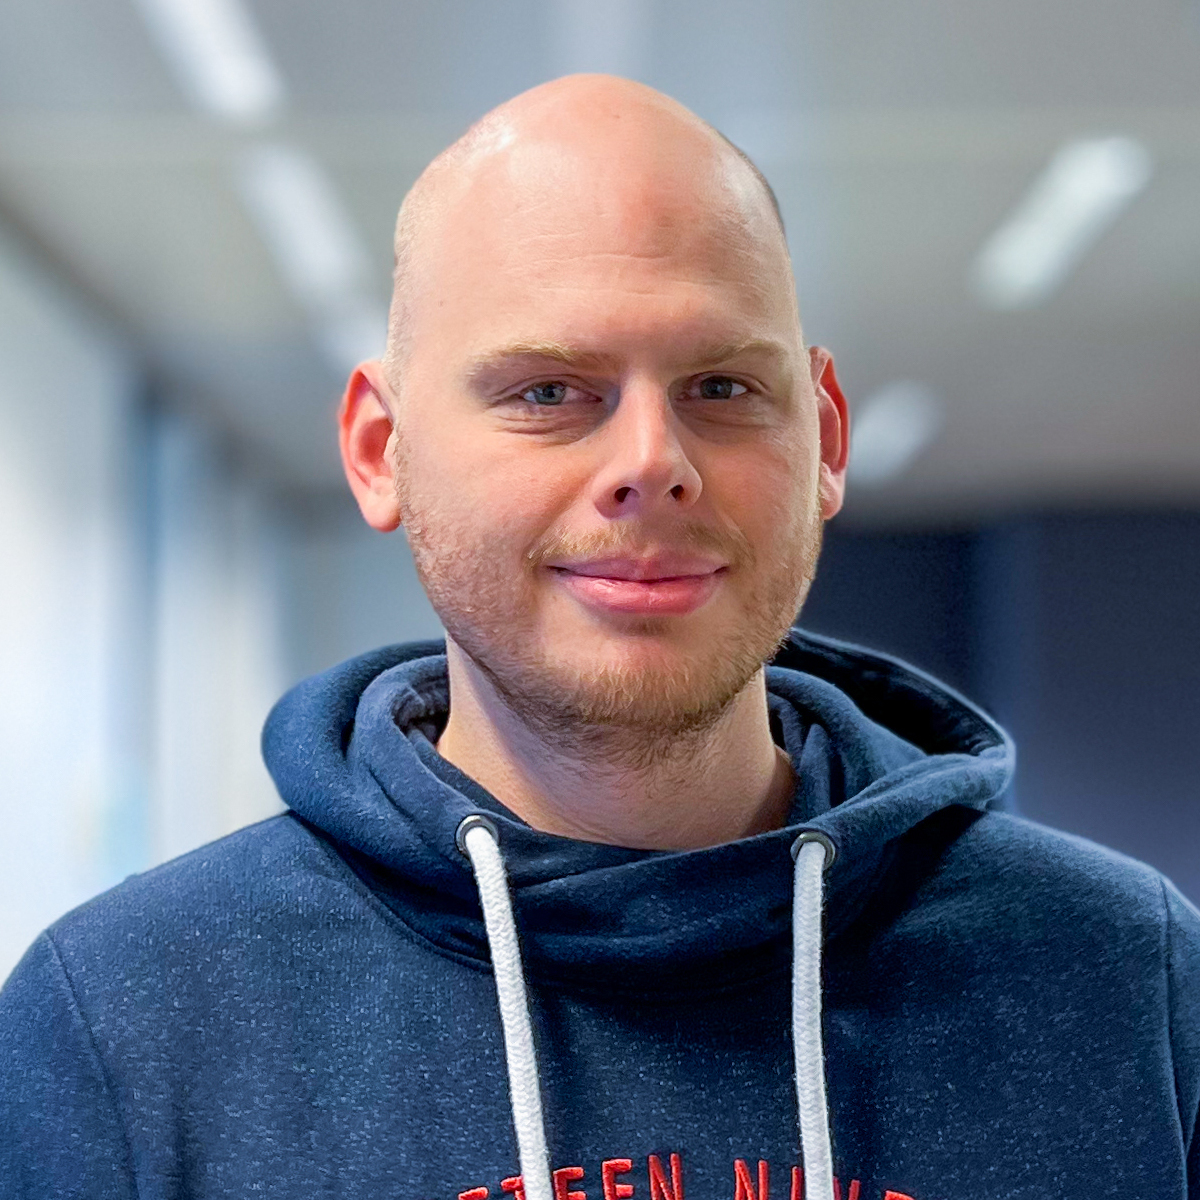
\includegraphics[width=2.8cm]{images/square.jpg}
}
\end{tabularx}
\begin{center}
\begin{tabularx}{\linewidth}{@{}*{2}{X}@{}}
% left side %
{
    \csection{Professional experiences}{\small
        \begin{itemize}
            % \item \frcontent{AppTweak}{Frontend development full-time - Brussels}{Worked full time as a  frontend developer in a team following the agile methodology. Contributed to build a complex data driven web application using }
            %   {Nov 2022 - Present}
            \item \frcontent{Igloo}{Web development internship - Louvain-la-Neuve}{Worked fulltime as a front end developer both on site and remote. Practiced React, Next.js and script writing in TypeScript. Reviewed my work dayly with the tech leader. Drove to produce clean code.}
              {Feb 2022 - Jun 2022}
            \item \frcontent{Interparking}{Web development internship - Remote}{Attend to a web and mobile app build using React and React native inside an Agile methodology. Interactions  the web team, the mobile team as well as the back end leader. Involed to the development and the test phases through pair programming. International context.}
            {Apr 2021 - Jun 2021}
        \end{itemize}
    }
    \csection{Studies}{\small
        \begin{itemize}
            % item 1 %
            \item \frcontent{Web development night classes}{IFAPME of Charleroi}{}{2020 - 2022}
            \item \frcontent{Bachelor AESI in Mathematics}{ENCBW in Louvain-la-Neuve}{}{2016 - 2020}
        \end{itemize}
    }
    \csection{Student jobs}{\small
        \begin{itemize}
            % item 1 %
            \item \frcontent{Volleyball coach}{Training and coaching multiple teams a year. Coordinating sports training camps. Managing kids, teenagers and adults.}{}{2014 - 2022}
            % item 2 %
            \item \frcontent{Bartender at la Clef de Verre}{Handeling bar and tables service}{}{2016 - 2017}
        \end{itemize}
    }
} 
% end left side %
& 
% right side %
{
    \csection{Development skills}{\small
        \begin{itemize}
            \item \textbf{Languages} \newline
            {\footnotesize TypeScript (JavaScript ES6+), Rust, PHP, HTML5 , CSS3 and SQL}{}{}
            \item \textbf{Practice, Library \& Framework} \newline
            {\footnotesize React, React-Native, Redux (RTK and Saga), Jest.js, Puppeteer, NodeJs, Express, Tailwind, Sass and Prisma }
            \item \textbf{Tools} \newline
            {\footnotesize Git, GitHub, Docker, Figma, Concourse CI, Vim and Linux}
        \end{itemize}
    }
    \csection{Soft skills}{\small
        \begin{itemize}
            \item Autonomous and self-thaught
            \item Problem solver
            \item Dynamic
        \end{itemize}
    }
    \csection{Languages}{\small
        \begin{itemize}
            \item {\footnotesize French native}
            \item {\footnotesize English C1}
        \end{itemize}
    }
    \csection{Interests}{\small
        \vspace{0.32cm}
        \begin{itemize}
            \item Volleyball
            \item Chess
        \end{itemize}
    }
    \csection{Contact}{\small
        \vspace{0.32cm}
        \begin{itemize}
            \item Linkedin: \href{https://www.linkedin.com/in/jp-roisin}{jp-roisin} 
            \item GitHub: \href{https://github.com/jp-roisin}{jp-roisin} 
        \end{itemize}
    }
}
\end{tabularx}
\end{center}
\end{document}
